\chapter{Antecedentes y estado del arte}\label{Antecedentes}
\section{Definición}
Se llama realidad aumentada al conjunto de tecnologías que permite a un usuario ver en tiempo real contenido virtual superpuesto al mundo real mediante un dispositivo tecnológico. El objetivo de esta tecnología es simplificar y facilitar el trabajo de los humanos en ciertos sectores, y gracias al increíble crecimiento que se está dando en el desarrollo de la realidad aumentada, sobre todo en los dispositivos móviles, la convierte en una tecnología muy barata y accesible. A diferencia de la realidad virtual, la realidad aumentada no sustituye la realidad, sino que la complementa para ayudar a comprender mejor el entorno en el que nos rodea.

\section{Historia}
\begin{wrapfigure}{r}{0.5\textwidth}
    \centering
    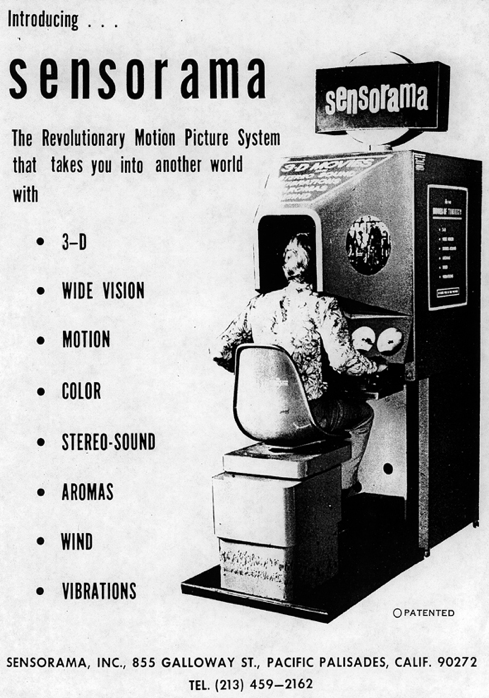
\includegraphics{Images/Sensorama.png}
    \caption{Cartel publicitario de la máquina Sensorama}
    \label{fig:Sensorama}
\end{wrapfigure}

En la década de 1950, surgió por primera vez el término realidad aumentada cuando Morton Heilig, cinematógrafo estadounidense, pensó en un prototipo de cine que estimulara todos los sentidos del ser humano de manera efectiva, de modo que la experiencia de cine fuera más completa. Años más tarde, concretamente en 1962, Heilig construyó dicho prototipo, al que llamó Sensorama. Se trataba de un cine inmersivo y novedoso que incluía funcionalidades como 3D, visión angular (actualmente conocido como IMAX), vídeo en color, sonido en estéreo, además de estimular otros sentidos con aromas, viento, y vibraciones~(figura~\ref{fig:Sensorama}). En la actualidad, estas funcionalidades están disponibles en algunos cines, por ejemplo la sala 4DX de Kinépolis \cite{kinepolis}.\\
\\
\\
\\


\begin{wrapfigure}{r}{0.5\textwidth}
    \centering
    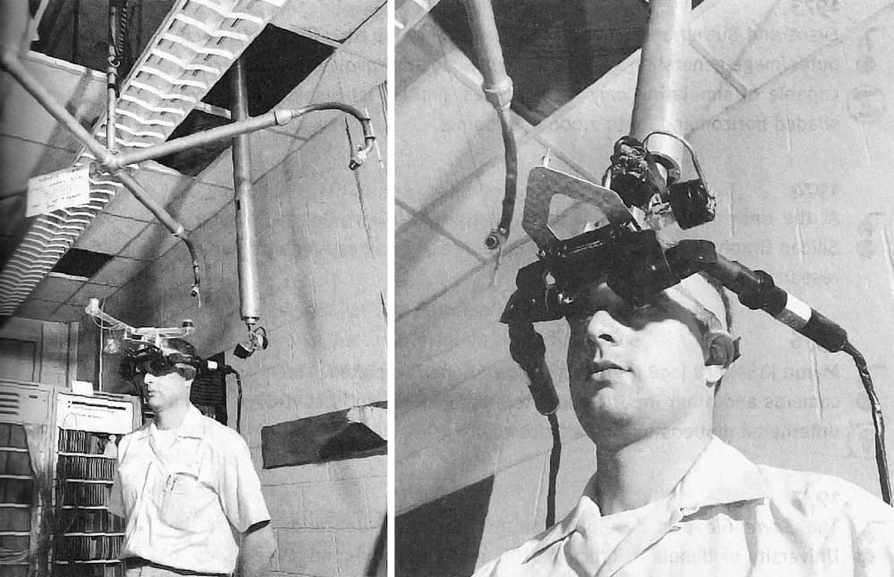
\includegraphics[width=0.48\textwidth]{Images/HumanMountDisplay.png}
    \caption{Ivan Sutherland ``Espada de Damocles'' 1968.}
    \label{fig:EspadaDamocles}
\end{wrapfigure}

 El HMD (\textit{Human Mounted Display}) se inventó en 1968 por Ivan Sutherland, fue el primer sistema que permitía ver en tiempo real las aristas de sencillos objetos 3D (\textit{Wireframe}) superpuesto al mundo real. Empleaba dos sistemas de \textit{tracking} para calcular el registro de la posición y rotación de la cámara; uno mecánico y otro basado en ultrasonidos. Debido a su gran peso se ancló el artefacto al techo, lo que le dio un aspecto característico que inspiró su nombre ``Espada de Damocles''~(figura~\ref{fig:EspadaDamocles}). Gracias a este dispositivo Sutherland pasó a la historia como uno de los pioneros de los cascos de realidad aumentada.\\

Sin embargo, no fue hasta 1992 cuando se acuñó el término de realidad aumentada tal y como lo entendemos hoy en día por Tom Caudell y David Mizell. Dos ingenieros de Boeing que proponían el uso de esta novedosa tecnología para mejorar la eficiencia y experiencia de las tareas realizadas por operarios humanos asociadas a la fabricación de~aviones.\\

La aparición del primer videojuego en realidad aumentada ocurrió en el año 2000. Bruce Thomas demostró en el ISWC (\textit{International Symposium on Wearable Computers}) su videojuego ARQuake. El sistema empleaba una brújula digital, un receptor de GPS y métodos de visión basados en marcas \cite{ARToolkit}. Los jugadores tenían que llevar una especie de ordenador portátil a la espalda, un casco de visión estereoscópica\footnote{ Dos puntos de vista poco separados entre sí.} y un mando de dos botones~\cite{ARQuake} (figura~\ref{Disp_ARQuake}). El funcionamiento del HMD (figura~\ref{HIWARQuake}) consistía en un divisor de haz que recibía la imagen virtual desde una pantalla que permitía ver el mundo real y el virtual en los ojos del usuario. La imagen resultante (figura~\ref{VisualizacionARQuake}) permitía una inmersión muy lograda para la época.

\begin{figure}[H]
\centering
\subfigure[Dispositivo utilizado \label{Disp_ARQuake}]{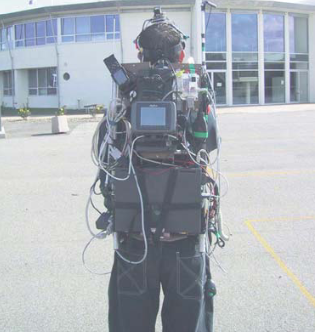
\includegraphics[width=0.32\linewidth]{Images/ARQuake_Dispositivo.png}}
\subfigure[Funcionamiento del HMD \label{HIWARQuake}] {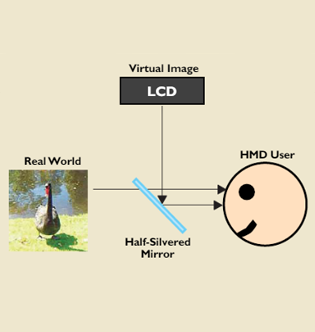
\includegraphics[width=0.32\linewidth] {Images/ARQuake_HIW.png}}
\subfigure[Visualización del videojuego\label{VisualizacionARQuake}]{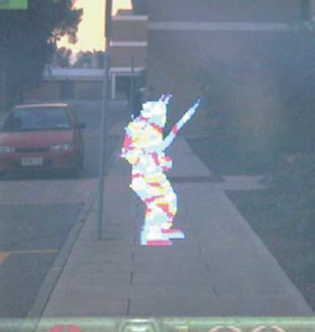
\includegraphics[width=0.32\linewidth]{Images/ARQuake_Example.png}}
\caption[ARQuake]{ARQuake~\cite{ARQuake}}\label{fig:ARQuakeFig}
\end{figure}


En 2007, en el ISMAR (\textit{International Simposium on Mixed and Augmented Reality}), Klein y Murray presentaron el sistema de \textit{tracking} PTAM (Parallel Tracking and Modeling) una variante al SLAM, que separa la localización y el mapeado en hilos diferentes. El SLAM, descrito en detalle en la sección~\ref{SLAMsection} es una tecnología que sirve para que localizar la posición dentro de un entorno y modelarlo. Separar estos dos procesos en hilos diferentes permitía conseguir unos resultados en tiempo real muy sólidos.\\

\begin{wrapfigure}{r}{0.6\textwidth}
    \centering
    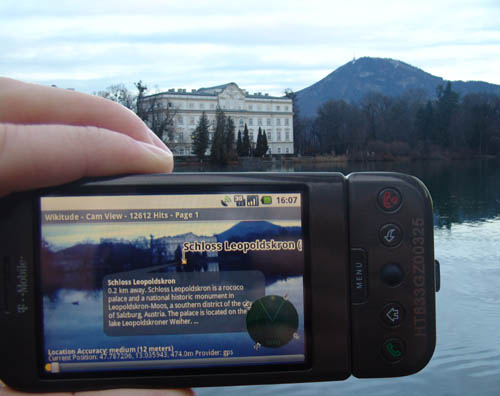
\includegraphics[width=0.4\textwidth]{Images/Wikitude_Example.jpeg}
    \caption[Wikitude App 2008]{Wikitude App 2008~\cite{ARToolkit}.}
    \label{fig:wikitude2008}
\end{wrapfigure}

En 2008 se creó Wikitude, una aplicación que utilizaba el GPS para mostrar al usuario información de la Wikipedia según el lugar en el que estuviese, pudiendo obtener datos sobre monumentos, esculturas o construcciones que estuvieran cerca. La aplicación (figura~\ref{fig:wikitude2008}) permite al usuario enfocar con la cámara del dispositivo obteniendo información como es el nombre del castillo, su origen, y la distancia a la que está.\\

Un año más tarde, en 2009, desarrolló el videojuego ARhrrrr!, del género shooter. El primer videojuego en realidad aumentada para \textit{smartphone} con contenido 3D de alta calidad. Se generaba un mapa 3D sobre un marcador, y el objetivo era rescatar a los humanos de la ciudad y matar a los zombies (figura~\ref{fig:arhrrrr})\cite{ARToolkit}.

\begin{figure}[H]
    \centering
        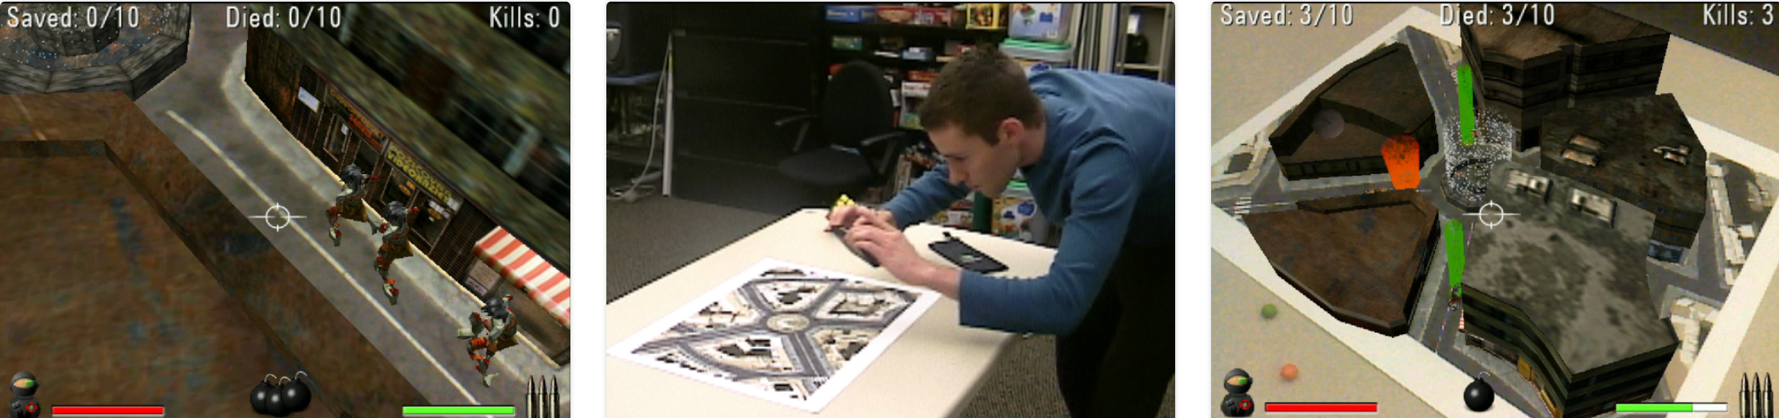
\includegraphics[width=\linewidth]{Images/Arrrr.png}
        \caption[Ejemplo del videojuego ARhrrrr!]{Ejemplo del videojuego ARhrrrr!\footnotemark.}
        \label{fig:arhrrrr}
\end{figure}

\footnotetext{Imagen sacada de \url{https://github.blairmacintyre.me/site-archive/ael-2015/research/games/arhrrrr/}}

En el mismo año, el estudio español Novorama creó el videojuego Invizimals, un juego de PSP (PlayStation Portable) que se convirtió en un éxito mundial, vendiendo más de 8 millones de copias en todo el mundo en el primer trimestre de 2010. Necesitaba usar la cámara adicional que se conectaba a la PSP, y gracias al uso de los marcadores, se podía registrar la posición del jugador.\\

En 2014 nació Project Tango, uno de los primeros desarrollos de realidad aumentada pensado para ser distribuido mundialmente en los \textit{smartphones}. En 2015, Tango pasó a formar parte de Google. El objetivo era mapear espacios tridimensionales usando solamente un dispositivo portátil. Esta tecnología sólo se desarrolló para el dispositivo Phab2 Pro de Lenovo, el cual incluía 3 cámaras, algo inusual en aquel momento.
Las tres funcionalidades principales para el desarrollo de esta tecnología han sido:
\begin{itemize}
\item Seguimiento del movimiento: Se trata del uso de las características visuales del entorno combinadas con los datos proporcionados por los sensores de movimiento incorporados en el teléfono, el acelerómetro y por el giroscopio, teniendo como objetivo realizar un seguimiento de los movimientos hechos del dispositivo. 
\item Reconocimiento del ambiente: Tango almacena la información del entorno que le rodea, buscando los puntos característicos en cada fotograma que recibe de las cámaras usando tecnologías explicadas con más detalle en la sección \ref{tecnologiasImplicadas}.
\item Percepción de profundidad: Gracias a las cámaras especiales que incorpora el dispositivo, Tango podía calcular tamaños y distancias en el entorno que se encuentra. 
\end{itemize}
Después de 3 años, en 2017, Google decidió cerrar el desarrollo de Tango y se centró en su tecnología actual, ARCore (sección~\ref{ARCore_Sec}), que es el competidor directo de ARKit (sección~\ref{ARKit_Sec}), la librería de Apple.

\newpage
\section{Dispositivos}
A principios de la década de 2010 las empresas más importantes de software y hardware empezaron a interesarse en el desarrollo de dispositivos que permitiesen el uso de aplicaciones de realidad aumentada sin tener que recurrir a móviles o \textit{tablets}. De esta forma, el uso de la realidad aumentada sería mucho más cómodo y abriría la puerta a un mundo completamente nuevo de posibilidades que hasta entonces eran desconocidas. 

\subsection{Google Glass}
Uno de los primeros proyectos de hardware para realidad aumentada fueron las Google Glass, impulsadas por Google, que fueron presentadas por primera vez en abril de 2012. El prototipo (figura~\ref{fig:GlassProt}) consta de una montura de gafas sin cristales, que en su patilla derecha incorpora una cámara y un pequeño procesador que permite la superposición de imágenes virtuales sobre lo que está viendo realmente el usuario. Aunque el diseño ha ido variando a lo largo de los años con las diferentes generaciones de Google Glass, el modelo ha mantenido la misma funcionalidad y se ha ampliado con nuevas prestaciones.\\

\begin{figure}[H]
     \centering
     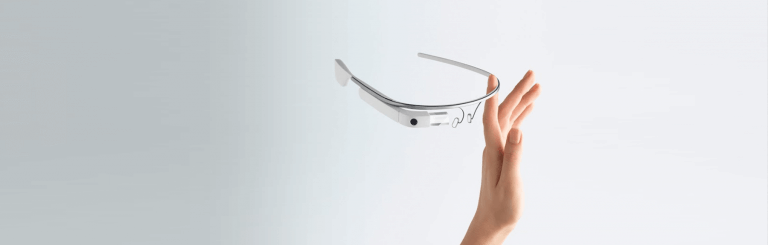
\includegraphics[width=0.7\linewidth]{Images/prototyping-google-glass-apps-768x245.png}
     \caption[Prototipo original de Google Glass]{Prototipo original de Google Glass\footnotemark}
     \label{fig:GlassProt}
 \end{figure}
 \footnotetext{Imagen sacada de \url{https://www.justinmind.com/blog/prototype-google-glass-applications}}

Google empezó a comercializar las gafas al año siguiente bajo el título de Glass Explorers al precio de 1500 dólares. Su público objetivo eran los desarrolladores, a los que se facilitó enormemente su labor con el fin de expandir los límites del nuevo hardware. Sin embargo, debido a que el dispositivo tomaba imágenes del mundo real y podía guardarlas y procesarlas se enfrentó a diversos problemas de privacidad. Una de las medidas que se tomaron por aquel entonces fue no aprobar ninguna aplicación que utilizase reconocimiento facial.\\

Ya en mayo 2014 salió a la venta para todos los públicos en Estados Unidos, retrasándose un mes en llegar a Europa. Las principales prestaciones que presentaba el dispositivo consistían en la consulta de mensajes, imágenes y otro tipo de datos presentes en los móviles sin necesidad de utilizarlos, poder consultar internet, siempre que se dispusiera de conexión, mediante órdenes de voz y grabar vídeo a una resolución de 720 píxeles~\cite{GlassAlm}.\\

Con el paso del tiempo y debido en parte a la falta de aplicaciones y a los problemas con la privacidad las gafas empezaron a fracasar en el mercado. Sin embargo Google cambió de estrategia y redirigió el objetivo de su producto. En 2017, las Google Glass Enterprise fueron presentadas y salieron a la venta, pero ahora se vendían a grandes empresas para facilitar el trabajo a sus empleados y hacerlo más cómodo mientras ganaban eficiencia. Con estas gafas se puede compartir lo que está viendo un usuario con el resto, así como obtener información rápida para el despeño de cualquier actividad, minimizando las distracciones y ganando en productividad.\\

El último paso de este dispositivo se ha dado en 2019, con el anuncio de las Google Glass Enterprise Edition 2 (figura~\ref{fig:GlassEnter}), que mejora las prestaciones de sus antepasados añadiendo características como el uso de inteligencia artificial o incluyendo el nuevo procesador \textit{Snapdragon XR1}. Aún no se conoce su fecha de lanzamiento, pero se ha anunciado que su precio ahora rondará los 1000 dólares. Pese a todo, no están pensadas para el público masivo sino para continuar mejorando el rendimiento de los trabajadores de las empresas~\cite{Andro4All}.\\ 

\begin{figure}[H]
     \centering
     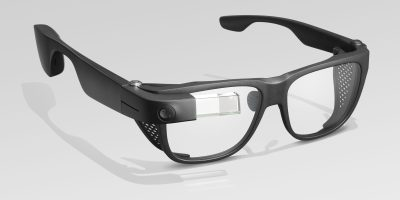
\includegraphics[width=0.6\linewidth]{Images/GlassEnterprise.jpg}
     \caption[Actuales Google Glass Enterprise 2]{Actuales Google Glass Enterprise 2\footnotemark}
     \label{fig:GlassEnter}
 \end{figure}
 \footnotetext{Imagen sacada de \url{https://www.google.com/glass/start/}}
 
\subsection{Hololens}
Microsoft, una de las empresas más importantes en el mundo del software, lanzó en el año 2016 su primer prototipo de gafas de realidad aumentada. Dicho prototipo, llamado Hololens, sólo se distribuía a desarrolladores y empresas por un precio de 3000\$. Se considera un HMD ya que son más grandes que unas simples gafas (figura \ref{fig:hololens}). Este dispositivo proyecta imágenes 3D sobre los cristales, permitiendo disfrutar de una experiencia de realidad aumentada. Incluso permite interactuar con los objetos con las manos gracias a la tecnología de Kinect\footnote{Tecnología de Microsoft lanzada en 2010 que se usaba en la Xbox. Incluía reconocimiento de voz y de gestos.}.

\begin{figure}[H]
\centering
\subfigure[Hololens 1\label{fig:Hololens1}] {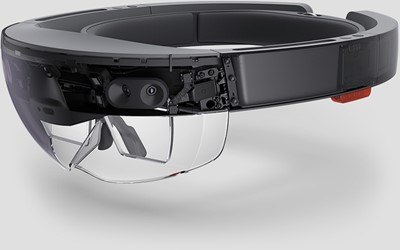
\includegraphics[width=0.44\linewidth]{Images/hololens.jpg}}
\subfigure[Hololens 2\label{fig:Hololens2}] {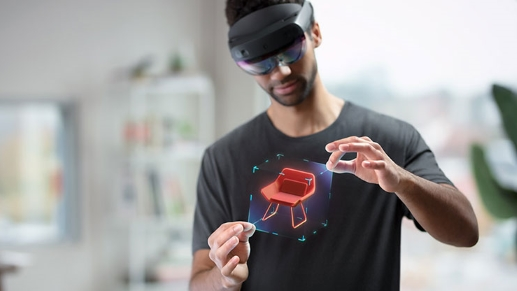
\includegraphics[width=0.49\linewidth] {Images/hololens2n.jpeg}}
\caption[Dispositivos Hololens]{Dispositivos Hololens\footnotemark}\label{fig:hololens}
\end{figure}
\footnotetext{Imagenes sacadas de \url{https://www.microsoft.com/es-es/hololens}}
 
Tres años más tarde, en el año 2019, Microsoft anuncia Hololens 2 (figura \ref{fig:Hololens2}), una versión mejorada de la misma que se puede obtener por 3500\$. Las posibilidades con este dispositivo son inquietantes. En su presentación, mostraron una demo que consistía en una conferencia a distancia, donde se veían hologramas de los usuarios remotos, y compartiendo la misma escena virtual. El reconocimiento de gestos permite interactuar con los objetos virtuales \cite{holovideo}. Está tecnología abre un sinfín de posibilidades para colaborar y trabajar con gente de forma remota.

\subsection{Magic Leap}
Magic Leap es una empresa estadounidense fundada por Rony Abovitz en 2010, su primer producto del mercado fueron las gafas Magic Leap One, dispositivo que prometió marcar un antes y un después en el mundo de los dispositivos de realidad aumentada. No fue hasta 2018 cuando empezó a distribuirse en Estados Unidos.\\

Las Magic Leap poseen un chip fotónico único en la industria, este chip permite modificar el espectro de luz generando imágenes nítidas ante nosotros. Gracias a esta tecnología prometedora, la empresa consiguió 3.000 millones de dólares de inversión y se declaró al dispositivo como futuro revolucionario~\cite{MagicLeap_AB}.\\

El producto está compuesto por una unidad principal con procesador y batería externo, unas gafas y un mando (figura~\ref{MagileapVisorMando}). Las gafas cuentan cámaras y sensores capaces de detectar el espacio en el que el usuario se encuentra. Sin embargo, este dispositivo posee un campo de visión muy reducido unos 50º frente a los 220º de visión de un humano. A pesar de esta limitación es uno de los dispositivos líderes en el mercado.

\begin{figure}[H]
\centering
\subfigure[Magic Leap One con su visor, unidad principal y mando.\label{MagileapVisorMando}] {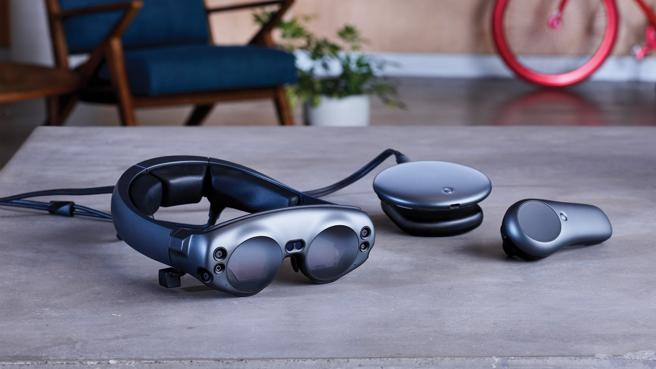
\includegraphics[width=0.635\linewidth]{Images/Magic_Leap_Gafas.jpg}}
\subfigure[Visualización en Magic Leap \label{MagicLeapHMD}] {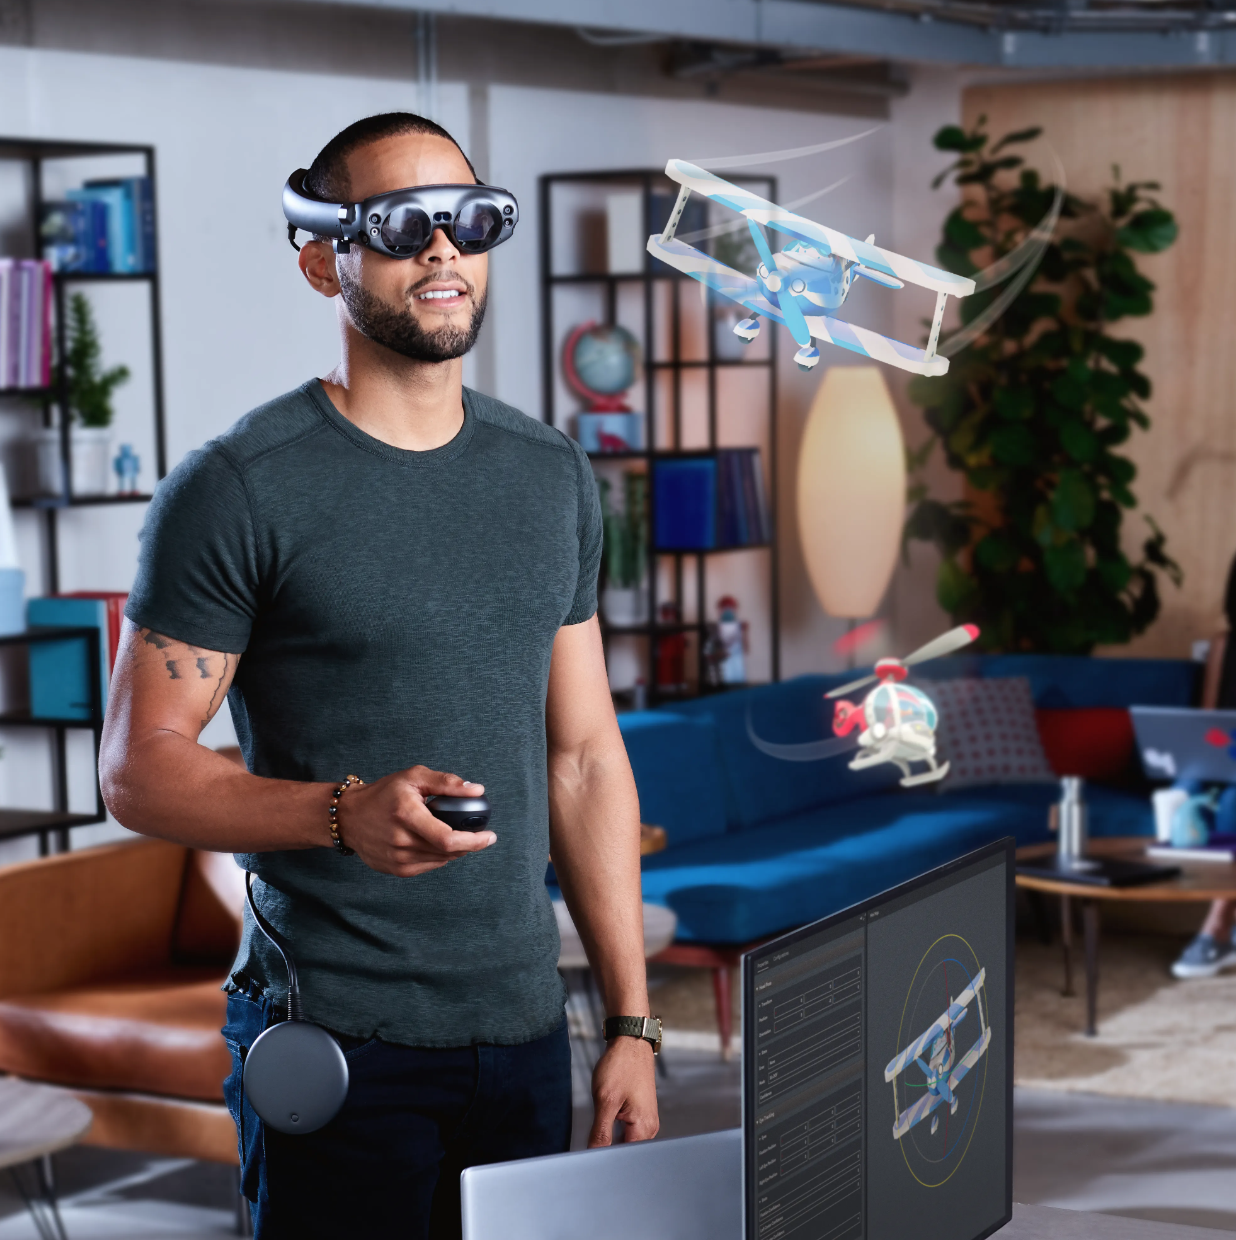
\includegraphics[width=0.355\linewidth] {Images/MagicLeapUso.png}}
\caption[Magic Leap]{Magic Leap\footnotemark}\label{fig:MagicLeap}
\end{figure}
\footnotetext{Imagen sacada de \url{https://www.magicleap.com}}

\subsection{Aryzon}\label{AryzonSection}
Las gafas de Aryzon son unas gafas estilo \textit{cardboard} de realidad aumentada compuestas por dos espejos que reflejan la imagen del \textit{smartphone} al cristal por donde nosotros vemos el mundo real, permitiendo tener esa visión de realidad aumentada (figura~\ref{GafasAryzon}). El funcionamiento es parecido al HMD que se usó en el año 2000 cuando se creó el ARQuake (figura~\ref{HIWARQuake}).

\begin{figure}[H]
\centering
\subfigure[Como funcionan las gafas Aryzon] {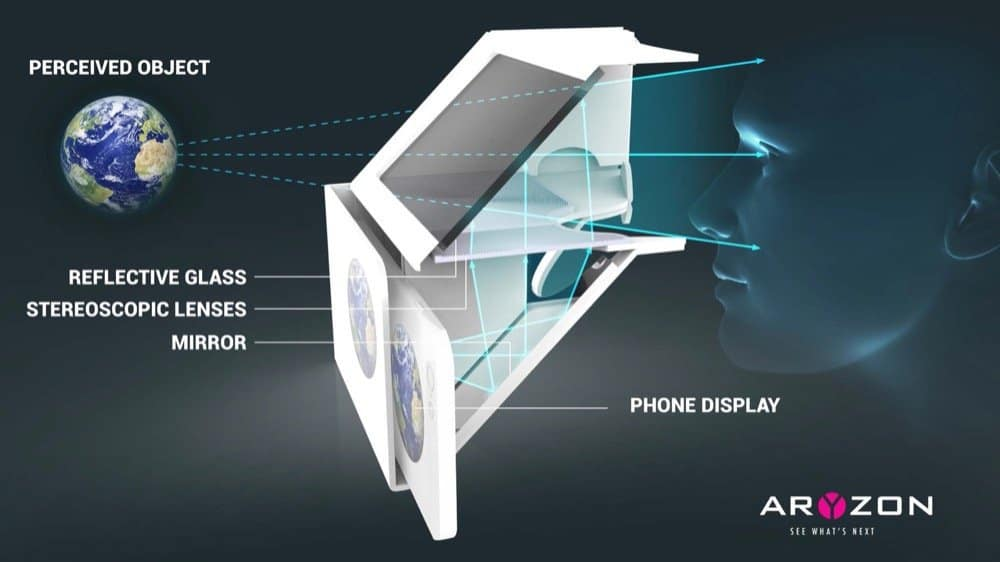
\includegraphics[width=0.47\linewidth]{Images/How-it-works.jpg}}
\subfigure[Ejemplo visualización Aryzon] {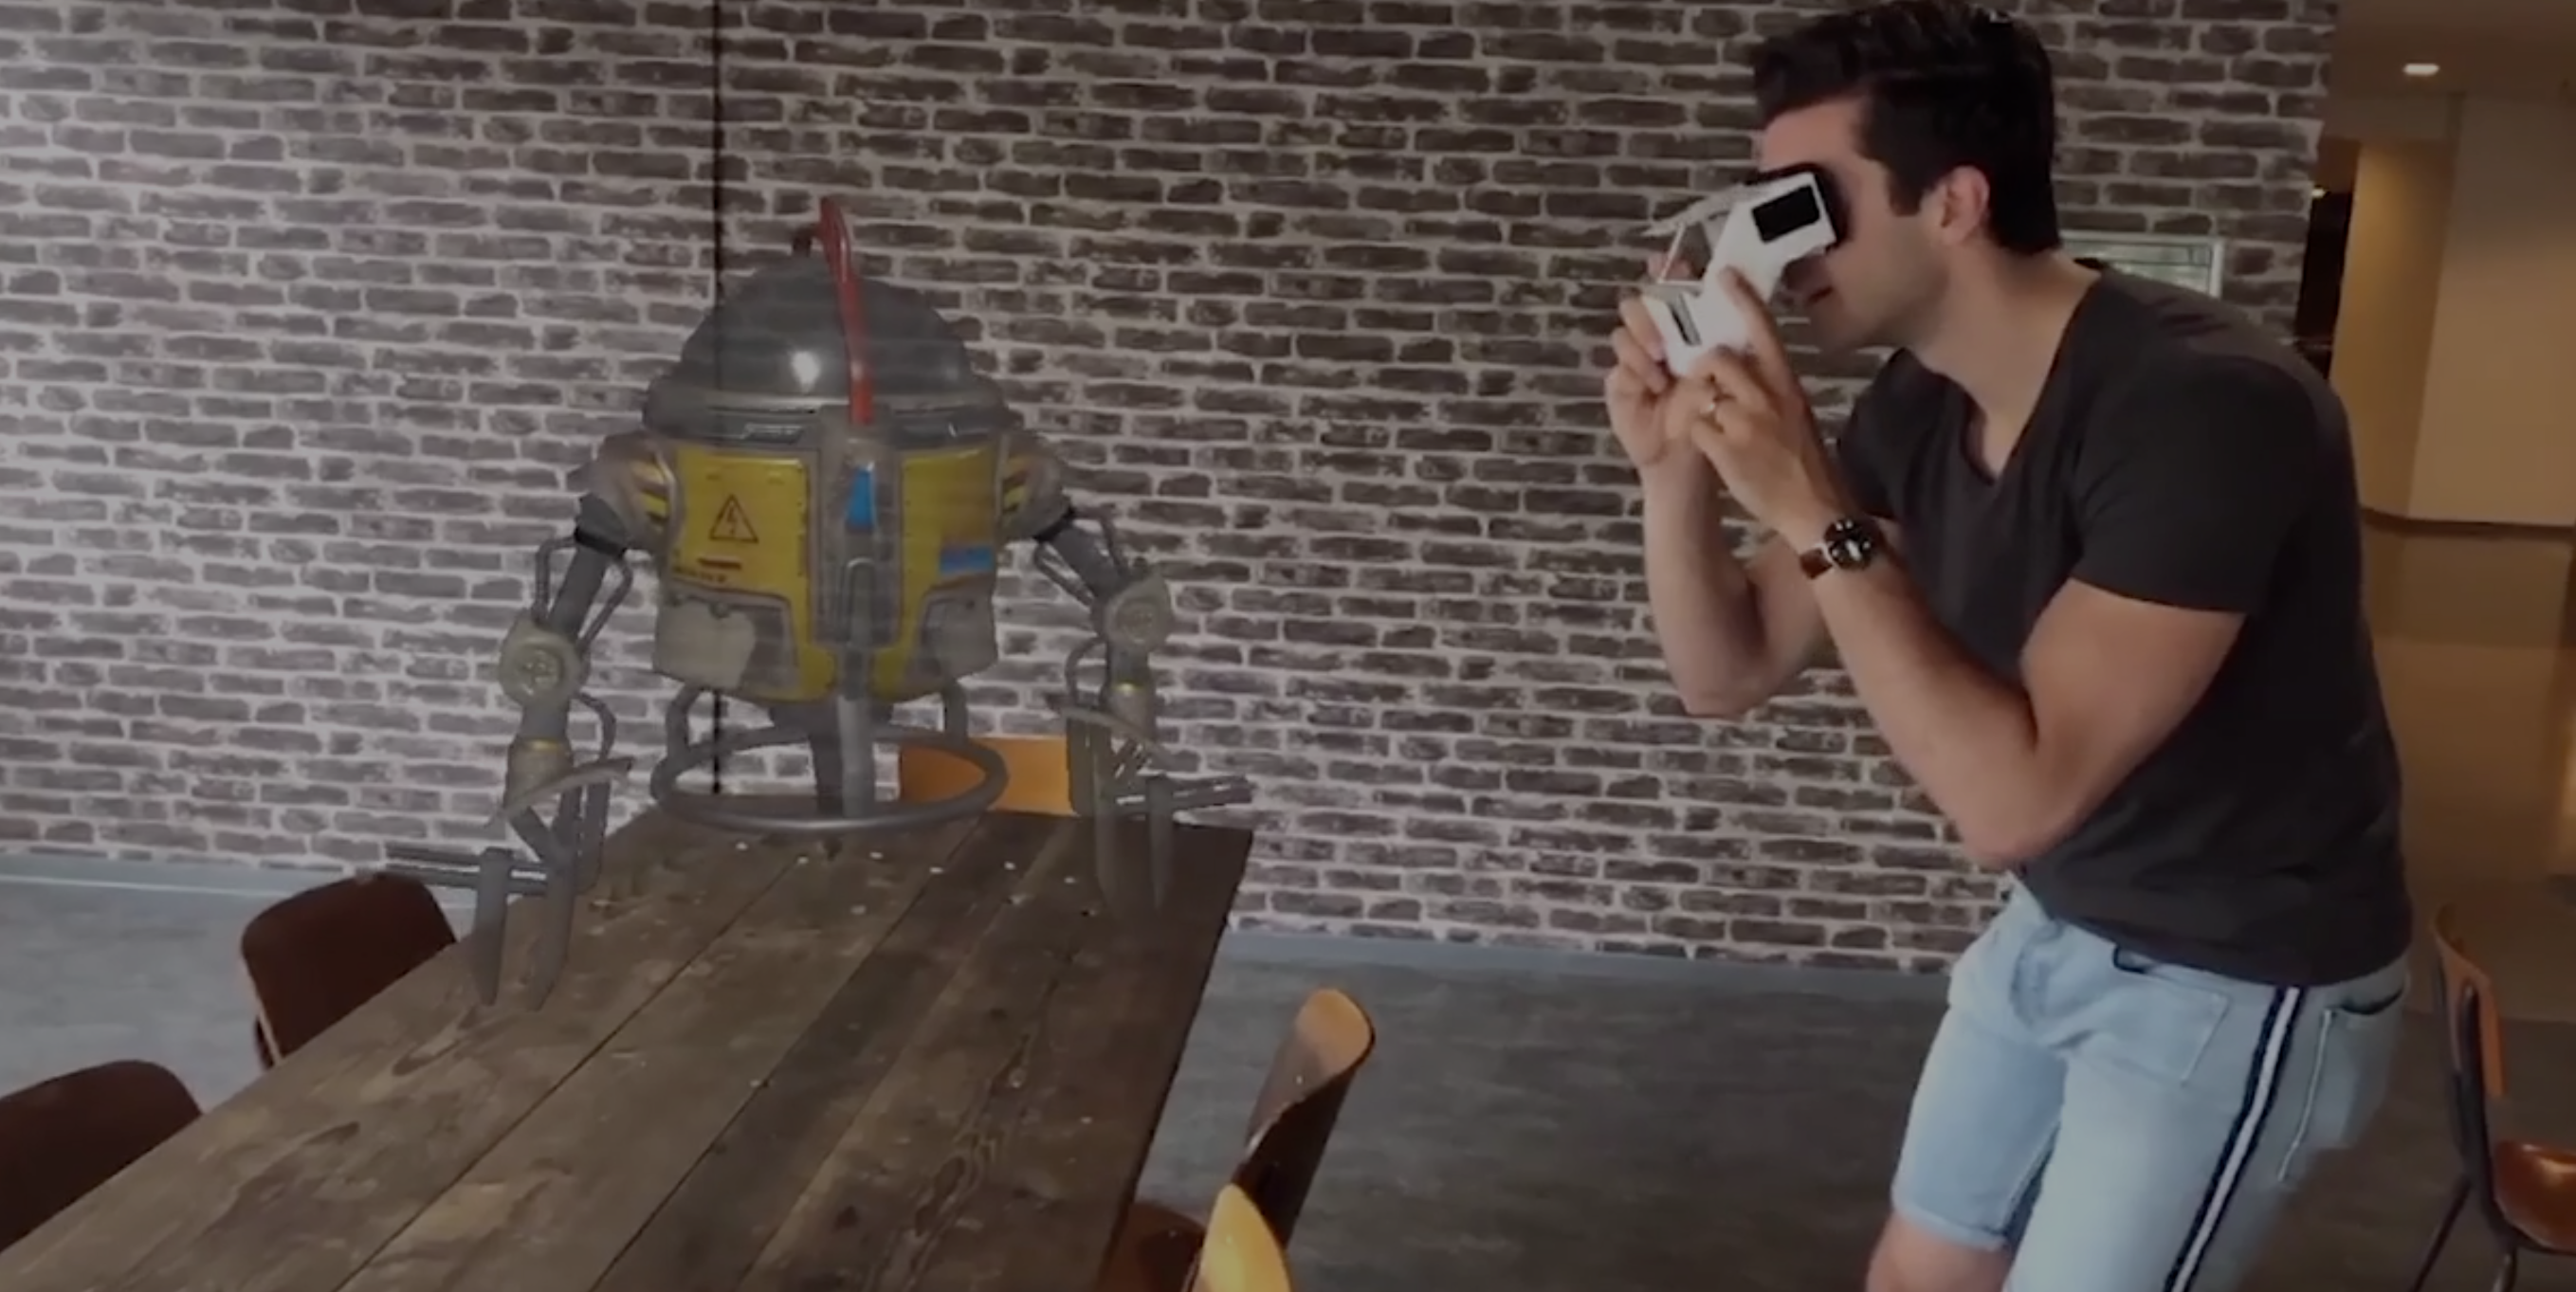
\includegraphics[width=0.52\linewidth]{Images/Aryzon_Demo.png}}
\caption[Gafas Aryzon]{Gafas Aryzon\footnotemark}\label{GafasAryzon}
\end{figure}
\footnotetext{Imagen sacada de \url{ https://www.igadgetsworld.com/aryzon-diy-augmented-reality-headset/}}


Estas gafas son accesibles para cualquier usuario, ya que cuestan 30€ y permiten disfrutar de la realidad aumentada sin necesidad de estar sujetando el móvil con la mano. La empresa proporciona un SDK donde te facilita el desarrollo de la aplicación, ya que se necesita una vista estereoscópica.
\newpage
\subsection{Otros dispositivos}
Los productos más destacados a día de hoy son las Google Glass, Hololens y Magic Leap, sin embargo también cabe nombrar dispositivos como Epson Moverio y Vuzix.\\

Las \textit{smartglasses} son un nicho de mercado de la realidad aumentada que revolucionará el mundo de la industria. Es por eso que las empresas tienen mucho interés en fabricar y desarrollar un producto con esta tecnología. Recientemente, Facebook ha confirmado la colaboración con la empresa de gafas Luxoticca para crear un dispositivo de realidad aumentada llamado Orion. Llevará integrado un asistente personal de Facebook y el objetivo principal es sustituir al teléfono móvil. Por otra parte, de manera paralela, está desarrollando un dispositivo llamado Agios, el cual tiene integrado un sensor de movimiento, que se sincronizará a las gafas para trabajar conjuntamente \cite{orion}.\\
Tras la salida del sistema operativo iOS 13, existen rumores de que Apple está trabajando en unas gafas de realidad aumentada, ya que han visto en el código y en la documentación referencias a un dispositivo de realidad aumentada \cite{applerumor}. Las especulaciones tienen unas expectativas muy altas, ya que ARKit (sección \ref{ARKit_Sec}) es una de las librerías líderes en la realidad aumentada para \textit{smartphones}.
\section{Aplicaciones}

En este apartado se recogen las principales aplicaciones por sectores que existen de la realidad aumentada. Estas son la medicina, educación, arte, seguridad, publicidad, turismo, e-commerce y videojuegos.\\
\subsection{Medicina}
El estrés intenso, incomodidad o la forma de vida sedentaria son factores que tienen un impacto negativo en el bienestar de las personas y su calidad de vida. Se han desarrollado numerosos prototipos para ayudar a la gente con este tipo de problemas. Por otra parte, las técnicas de \textit{gamificación}\footnote{ Técnica de aprendizaje que traslada mecánicas de los juegos al ámbito educativo-profesional con el fin de conseguir mejores resultados.} han sido usadas con éxito en aplicaciones cuyo fin es mejorar la salud de las personas incentivándolas a cambiar sus malos hábitos.\\

Además, ciertos conceptos de juegos de realidad aumentada pueden ser utilizados con propósitos de salud en ancianos. La actividad física es un aspecto clave al hacernos mayores. Algunas consideraciones conceptuales e investigaciones han ayudado a desarrollar entornos de realidad aumentada que sirvan a las personas mayores para hacer ejercicio y mejorar su calidad de vida.\\

Debemos mencionar también que además de ayudar a los pacientes, la realidad aumentada también es capaz de ayudar a los doctores, como podemos ver en la figura~\ref{fig:Surgeon}, los cirujanos se sirven de un programa que crea una proyección virtual sobre el cuerpo del paciente que funciona como guía en el transcurso de la operación.

\begin{figure}[H]
     \centering
     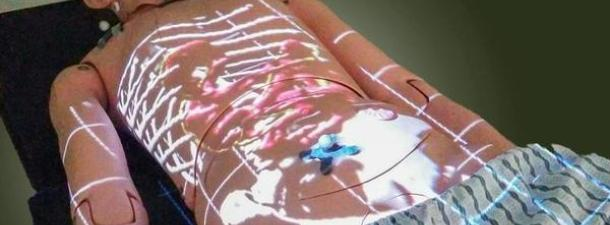
\includegraphics[width=0.7\textwidth]{Images/medicina_AR.jpg}
     \caption[Uso de realidad aumentada en una intervención quirúrgica]{Uso de realidad aumentada en una intervención quirúrgica\footnotemark.}
     \label{fig:Surgeon}
 \end{figure}
  \footnotetext{Imagen sacada de \url{https://i2.wp.com/blogthinkbig.com/wp-content/uploads/2018/04}}

Como éste, existen gran variedad de conceptos que implican el uso de la realidad aumentada para favorecer el bienestar y la calidad de vida de las personas~\cite{ARGames_Gamification}.\\
Una de las aplicaciones dignas de mención es Brain Power, un software que se vale de dispositivos de realidad aumentada como las Google Glass para favorecer la integración de personas con síndrome de Asperger. La aplicación propone una serie de desafíos a modo de juego que mejoran las habilidades sociales de los pacientes y mide su progreso periódicamente~\cite{RealAumento}.

\subsection{Educación}
Los juegos en realidad aumentada, en el sector de la educación, tienen el potencial de abrir el camino a nuevas formas de aprendizaje y adquisición de conocimientos, cambiando la experiencia del estudio. Aun así, todavía hay algunas dudas sobre cómo los juegos que utilizan la realidad aumentada pueden ser usados para expandir el proceso educativo convencional. Pese a este desconocimiento, es innegable que los métodos de aprendizaje basados en la gamificación y en el uso de la realidad aumentada han conseguido una mayor implicación de los estudiantes y un mayor interés por el aprendizaje de nuevas materias~\cite{ARGames_Gamification}.\\

Un ejemplo de ello es la aplicación Elements 4D, surgida en Kickstarter, que proporciona una nueva visión de los elementos químicos y facilita el aprendizaje con una parte narrativa y otra jugable (figura~\ref{fig:Elemets}).\\

\begin{figure}[H]
     \centering
     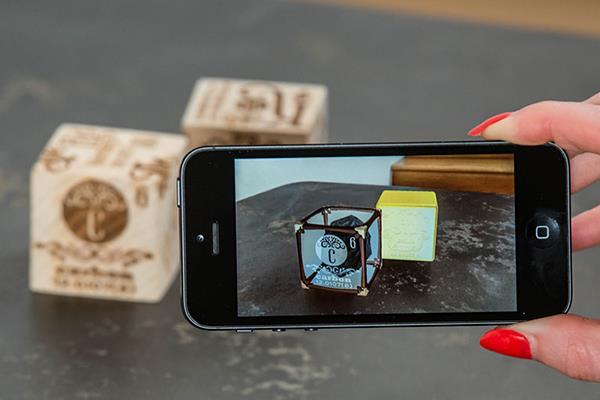
\includegraphics[width=0.5\textwidth]{Images/Figura-3-Elements-4D.png}
     \caption[Juego educativo Elements 4D]{Juego educativo Elements 4D\footnotemark}
     \label{fig:Elemets}
 \end{figure}
 \footnotetext{Imagen sacada de \url{https://www.researchgate.net/publication/317145820/figure/fig1/AS:498232876253185@1495799382235/Figura-3-Elements-4D-Fuente-http-crowdfundbeatcom.png}}
 
 Otra propuesta educativa, en este caso de la BBC, es Civilisations AR~\cite{Xat11Apps}. Consiste en un programa que emplea la realidad aumentada para representar diferentes objetos pertenecientes a civilizaciones y culturas del pasado con los que podemos interactuar. Además incluye funcionalidades como los rayos X, para explorar más a fondo, o guías audibles para obtener más información.\\
 
 También existen aplicaciones que utilizan la realidad aumentada para ayudar a aprender idiomas, como en el caso de Mondly~\cite{Xat11Apps}. La aplicación utiliza un profesor virtual proyectado sobre el mundo real así como otros muchos objetos que facilitan la asociación de los términos con su significado, permitiendo aprender hasta 33 idiomas en una experiencia nueva y gratificante.

\subsection{Arte}
El arte es un campo en constante transformación que se renueva cada año para transmitir emociones desconocidas y contar nuevas historias que permanezcan en el recuerdo de los espectadores. Como no podía ser de otra forma, los artistas de vanguardia han querido probar nuevas formas de creación con el uso de la realidad aumentada, elaborando obras híbridas que se valgan tanto del arte tradicional como de figuras y elementos virtuales que aportan una nueva capa de expresión y profundidad.\\

En ocasiones, estas obras permiten incluso la interacción del espectador. Este hecho es especialmente notable, ya que no sólo permite el paso de una experiencia pasiva a una activa, sino que a veces la propia obra permite la extensión de su arte, que es complementado por la visión y las acciones del que la ve.\\

Uno de los ejemplos más recientes es Mirages \& Miracles~\cite{elemmental}, una exposición de arte contemporáneo cuyo núcleo es la fusión de lo material y lo inmaterial, jugando con lo que consideramos real y falso. Los dibujos de la exposición han sido hechos a mano, pero con la ayuda de \textit{tablets} los espectadores pueden ver la obra al completo y ver lo que está más allá de la simple pintura, con figuras virtuales minimalistas y evocativas. Los artistas son Adrien Mondot y Claire Bardainne, cuyas últimas obras aspiran a ser arte digital vivo.

\begin{figure}[H]
     \centering
     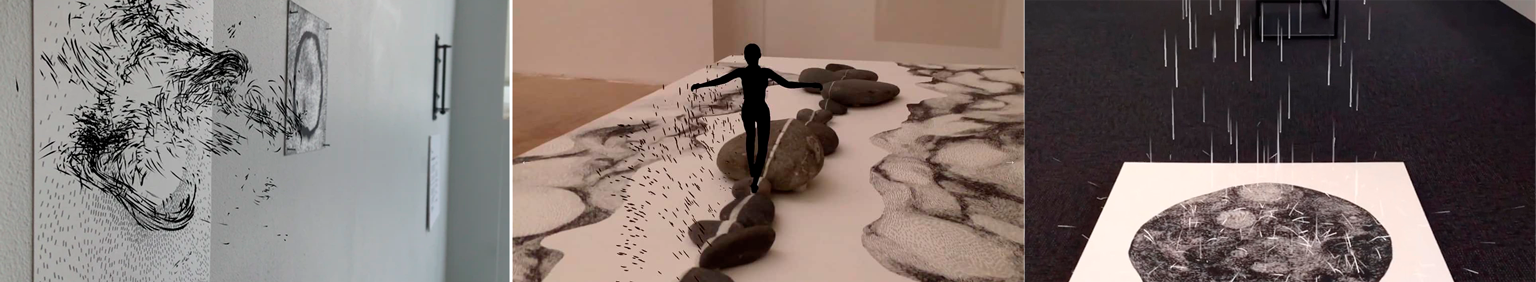
\includegraphics[width=\textwidth]{Images/AR-Art-Exhibition-Mirages-and-Miracles.png}
     \caption[Exhibición de Adrien M y Claire B \textit{Mirages and Miracles}]{Exhibición de Adrien M y Claire B \textit{Mirages and Miracles}\footnotemark.}
     \label{fig:Mirages and Miracles}
 \end{figure}
\footnotetext{Imagen sacada de \url{https://graffica.info/adrien-m-claire-b/}}

\subsection{Fabricación}
Con la constante mejora de la tecnología móvil y los múltiples avances en el campo de la realidad aumentada no sorprende la cantidad de aplicaciones con diferentes utilidades que podemos encontrar en el mercado. El sector industrial no es una excepción, siendo éste uno de los principales beneficiados por la evolución de este campo. De hecho, como comentábamos en la sección de historia, el término de realidad aumentada fue acuñado por dos trabajadores de este campo, ingenieros de Boeing, que utilizaban esta tecnología para facilitar la fabricación de aviones.\\

En la actualidad, valiéndose de estos sistemas, ya podemos empezar a hablar de fábricas inteligentes que mejoran la transmisión de información entre las máquinas y los operarios y permiten una mejor gestión de los recursos y de los datos disponibles, mejorando así la eficiencia y la productividad de forma drástica. Un ejemplo de ello está en el diseño industrial: disponiendo de las diferentes piezas virtuales, la realización de prototipos y el intercambio de los diferentes componentes es sumamente rápido y no tiene ningún impacto sobre otros modelos. Pero sus aplicaciones en una fábrica también se extienden al mantenimiento de la misma o incluso a la seguridad laboral~\cite{Neosentec_Fab}.\\ 

Otra de las principales aplicaciones en este terreno es la formación de los operarios mediante el uso de textos explicativos o imágenes que aparecen en realidad aumentada.\\

Se puede observar en la figura~\ref{fig:placenote} algunas de las aplicaciones en la industria, donde se puede señalar dónde hay una avería, o que hay que inspeccionar, muy útiles para compartir información entre trabajadores y evitar malentendidos.

\begin{figure}[H]
     \centering
     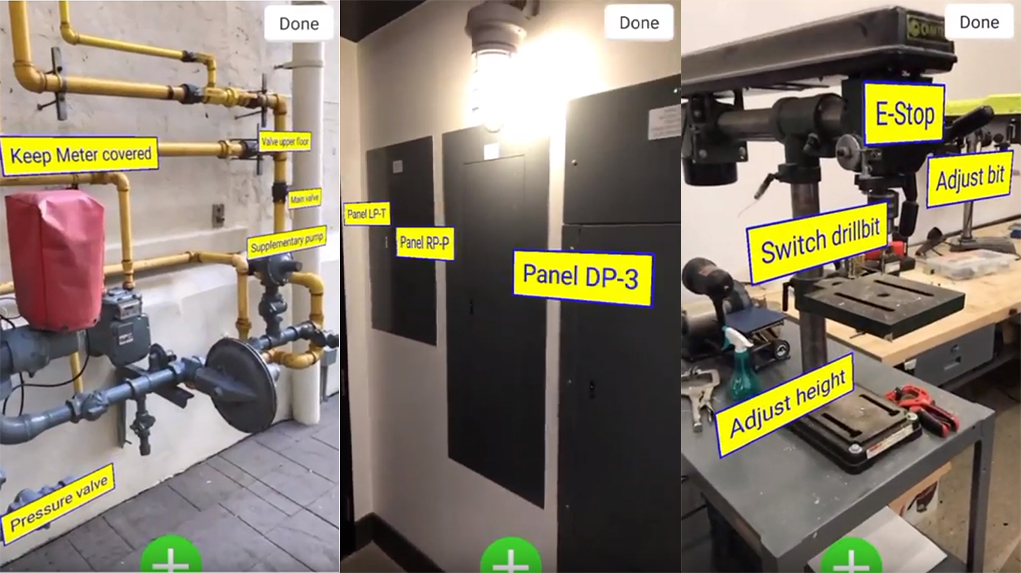
\includegraphics[width=0.7\textwidth]{Images/Placenote.jpg}
     \caption[Ejemplos de uso en la Fabricación]{Ejemplos de uso en la Fabricación~\cite{PlacenoteYT}.}
     \label{fig:placenote}
 \end{figure}
 
\subsection{Publicidad}
No es ningún secreto que el objetivo primordial de la publicidad es vender un producto a un comprador concreto. Desde el principio de los tiempos la publicidad ha sido agresiva y vistosa, con el fin de llegar a un público mayor y sorprender al que la presencia para que se plantee si necesita lo que se le está vendiendo. En los días que vivimos la publicidad se vale de todos los recursos que tiene a su alcance para ampliar sus horizontes, y la tecnología de la realidad aumentada no es excepción. Los anuncios y aplicaciones de realidad aumentada son especialmente exitosos, ya que el usuario no sólo está viendo la publicidad, sino que es partícipe de ella y puede sumergirse en la experiencia con todos sus sentidos.\\

Multitud de empresas han empezado a incorporar la realidad aumentada en sus diferentes anuncios. Un ejemplo de ello en el campo del motor son las aplicaciones de BMW, que permiten la interacción por parte de los clientes con modelos virtuales de sus productos, como coches u otros vehículos~\cite{Neosentec_Pub}.\\

Otro ejemplo del uso de esta tecnología en la publicidad es la idea de Burger King que se puede ver en la figura~\ref{fig:nikeAR}. Se trata de una campaña publicitaria que incentiva a los usuarios a “quemar” los carteles de la competencia mediante el uso de una aplicación móvil. Como recompensa por ello se recibe un cupón canjeable por una hamburguesa del Burger King~\cite{Designboom}.

\begin{figure}[H]
     \centering
     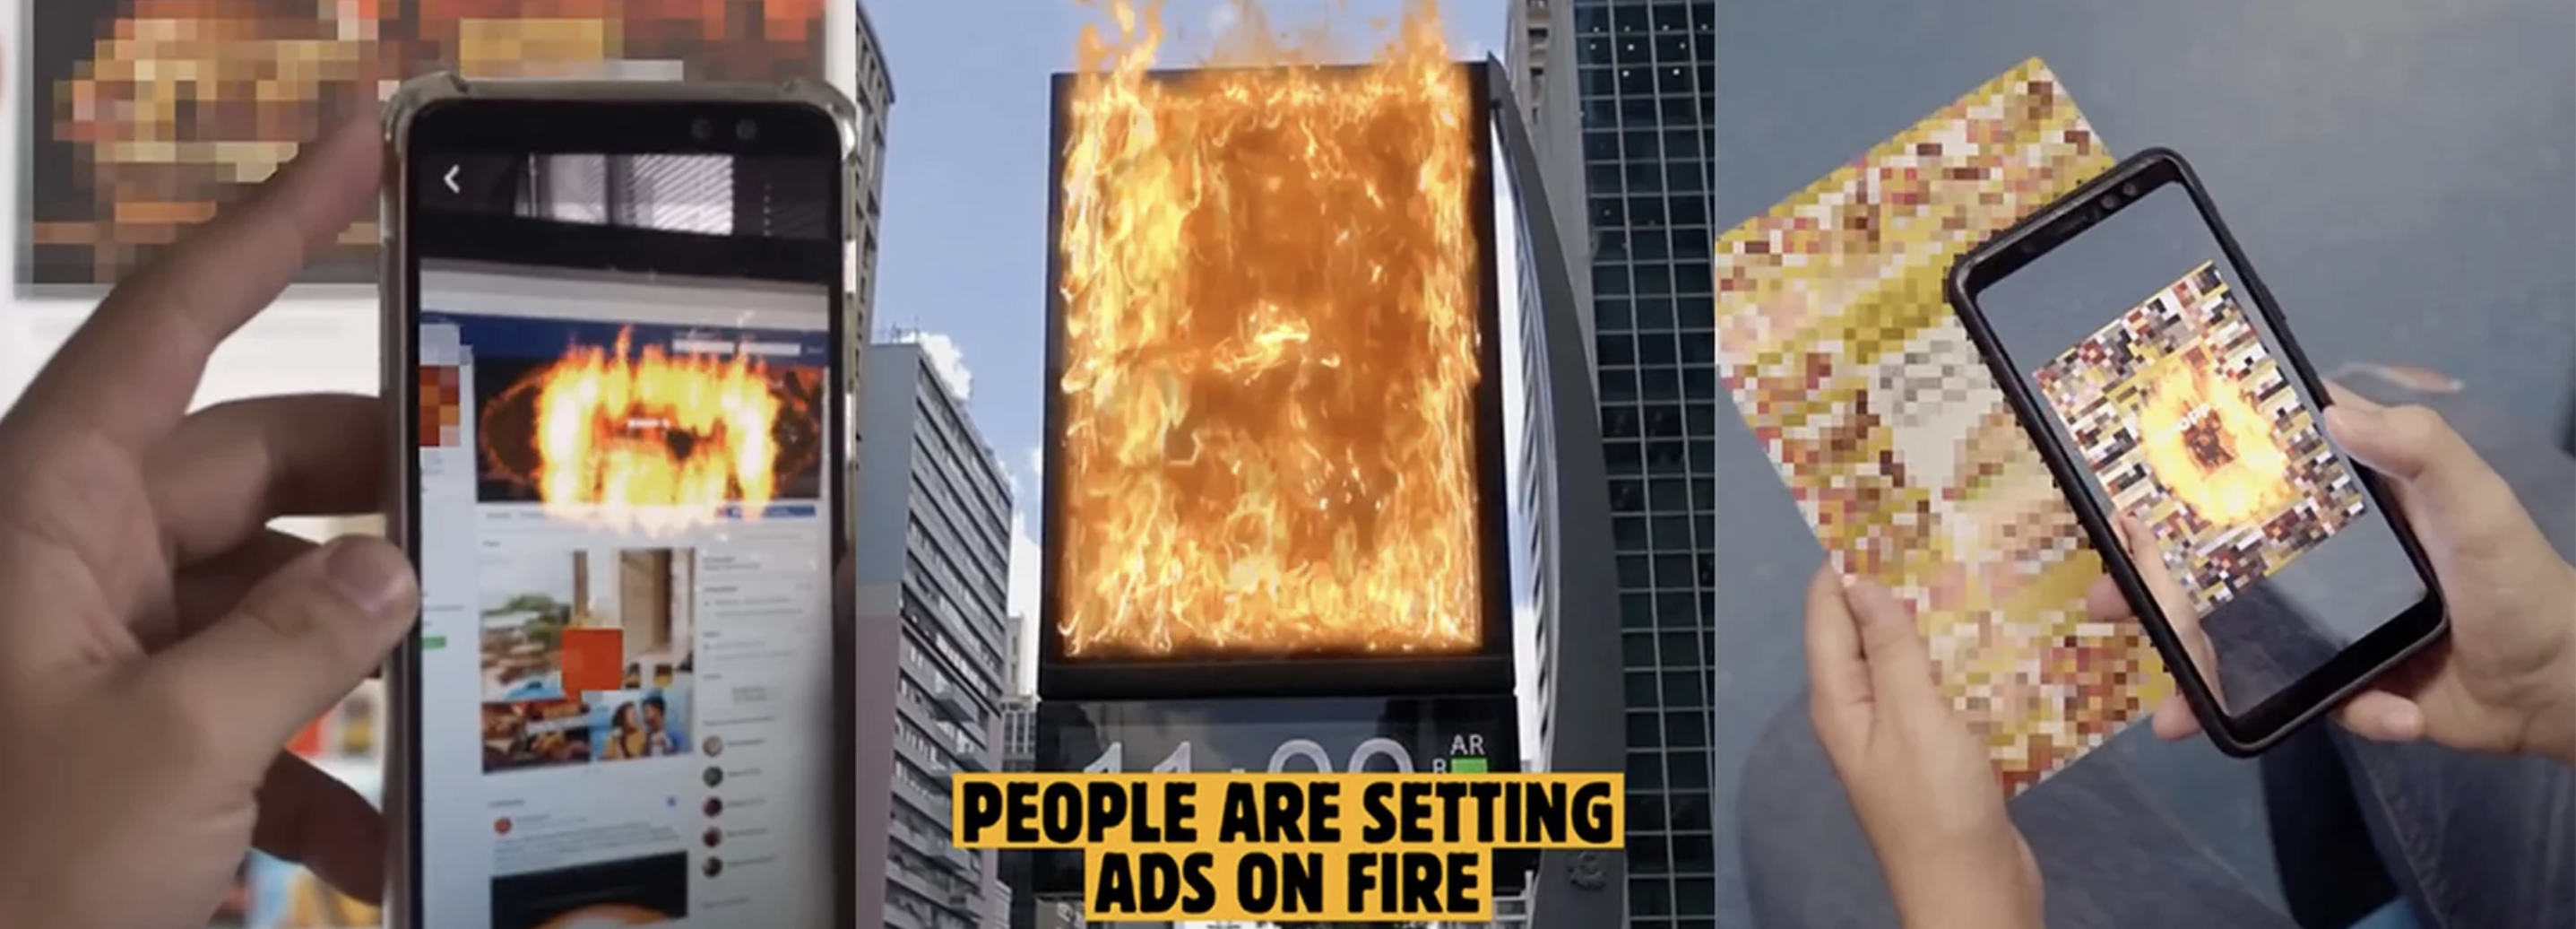
\includegraphics[width=\textwidth]{Images/BurgerKing_Add.png}
     \caption[Burger King campaña publicitaria]{Burger King campaña publicitaria\footnotemark.}
     \label{fig:nikeAR}
 \end{figure}
 
 \footnotetext{Imagen sacada de \\ \url{https://www.designboom.com/technology/burger-king-burn-that-ad-free-whopper-virtual-reality-03-21-2019/}}

\subsection{Turismo}
En los últimos años hemos podido encontrar un gran aumento en el desarrollo de aplicaciones de realidad aumentada. Esto se debe principalmente a que la tecnología cada vez es mejor, más barata y accesible, y permite disfrutar de este campo a muchas más personas y de una forma más directa e intuitiva. Precisamente es necesario diseñar aplicaciones intuitivas y sencillas si van a ir dirigidas a un público que no esté habituado al mundo digital; como es en el caso de las aplicaciones de realidad aumentada en el sector del turismo~\cite{Neosentec_Tur}.\\

Existen multitud de maneras en las que el usuario puede interactuar con el entorno en estas aplicaciones. Con esto el turista además de estar físicamente en un destino también puede interactuar con él, haciendo más completa su experiencia y obteniendo información o fuentes de ocio que de otras maneras habrían pasado inadvertidas. A día de hoy ya existen lugares como parques de atracciones que se valen de esta tecnología para guiar a los usuarios por el recinto y les ofrecen diferentes actividades y juegos para que su experiencia sea inolvidable. Un ejemplo de ello es el prototipo implementado por Lego para el parque Legoland Dinamarca. El usuario puede seguir a un guía virtual hecho de piezas Lego y previsualizar las atracciones antes de montarse~\cite{twitter_lego}.\\

\begin{figure}[H]
     \centering
     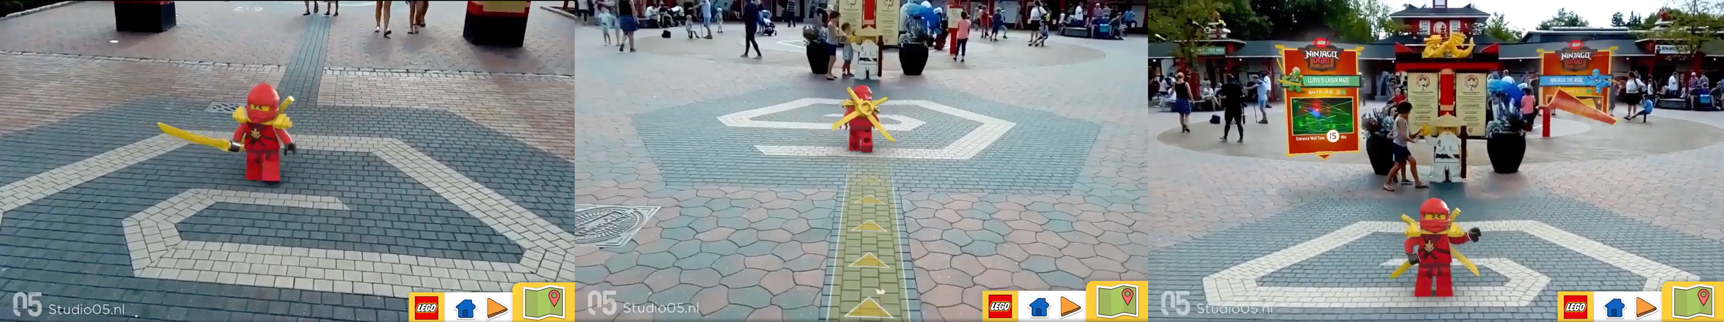
\includegraphics[width=\textwidth]{Images/Lego_Park.png}
     \caption[Aplicación para el parque Legoland]{Aplicación para el parque Legoland \footnotemark.}
     \label{fig:googletranslate}
 \end{figure}

\footnotetext{Imagen sacada de  \url{https://www.youtube.com/watch?v=gSTJmO9nMpU}}

\begin{wrapfigure}{r}{0.5\textwidth}
    \centering
    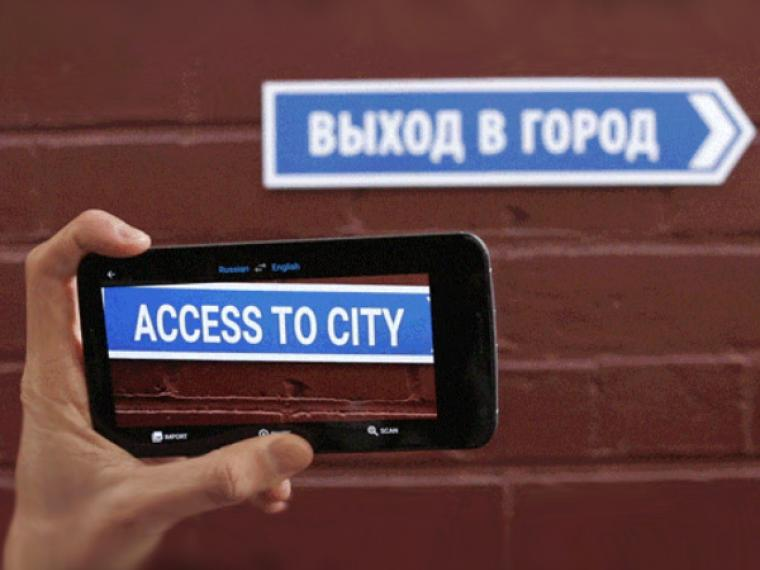
\includegraphics[width=0.5\textwidth]{Images/google-translate.jpg}
    \caption[Traductor de Google en RA]{Traductor de Google en RA\footnotemark.}
    \label{fig:googletranslate}
\end{wrapfigure}
 

Por supuesto, la realidad aumentada presenta otro beneficio primordial a la hora de viajar a otro país con una lengua diferente a la nuestra. Existen aplicaciones que con el uso de la cámara traducen en tiempo real carteles y cualquier tipo de texto de un idioma a otro. Como podemos observar en la figura~\ref{fig:googletranslate}, su uso es muy cómodo, sobre todo para los idiomas que no utilizan nuestro alfabeto, ya que no hace falta escribir el texto para traducirlo. Esto resulta increíblemente rápido y eficaz a la hora de obtener información y sin duda mejorará la experiencia turística en destinos internacionales.

\footnotetext{Imagen sacada de  \url{https://www.muyinteresante.es/tecnologia/articulo/el-nuevo-google-translate-traduce-imagenes-y-voz-211421238921}}
  


\subsection{Videojuegos}
El sector del ocio electrónico es en la actualidad más grande de lo que nunca ha sido. Se sabe que el dinero que mueve es mayor al que suman las industrias cinematográfica y discográfica juntas~\cite{libroblanco}, y no sorprende a nadie el hecho de que la realidad aumentada haya encontrado aquí el nicho perfecto en el que asentarse y desarrollarse.\\

El auge de la industria del videojuego viene impulsado en los últimos años por la accesibilidad de los móviles y el desarrollo de juegos para estos dispositivos. De hecho, la aplicación que permitió la difusión masiva al público general de la realidad aumentada fue Pokémon Go en 2016 (aunque ya lo había conseguido en menor medida Invizimals en 2009), que se convirtió en un fenómeno mundial durante el verano de dicho año y que este año ha experimentado otro pico de facturación que no se alcanzaba desde su lanzamiento~\cite{meristation_pokemonGo}. Una de las claves de su éxito fue innegablemente basarse en la conocida franquicia, sin embargo, cada ciertos años sale al mercado una nueva entrega de la saga principal en las consolas de Nintendo y no logra la difusión y fiebre masiva que sí consiguió esta aplicación, lo que nos sugiere que la realidad aumentada y la accesibilidad también son decisivos en el entusiasmo del público.\\

\begin{figure}[H]
     \centering
     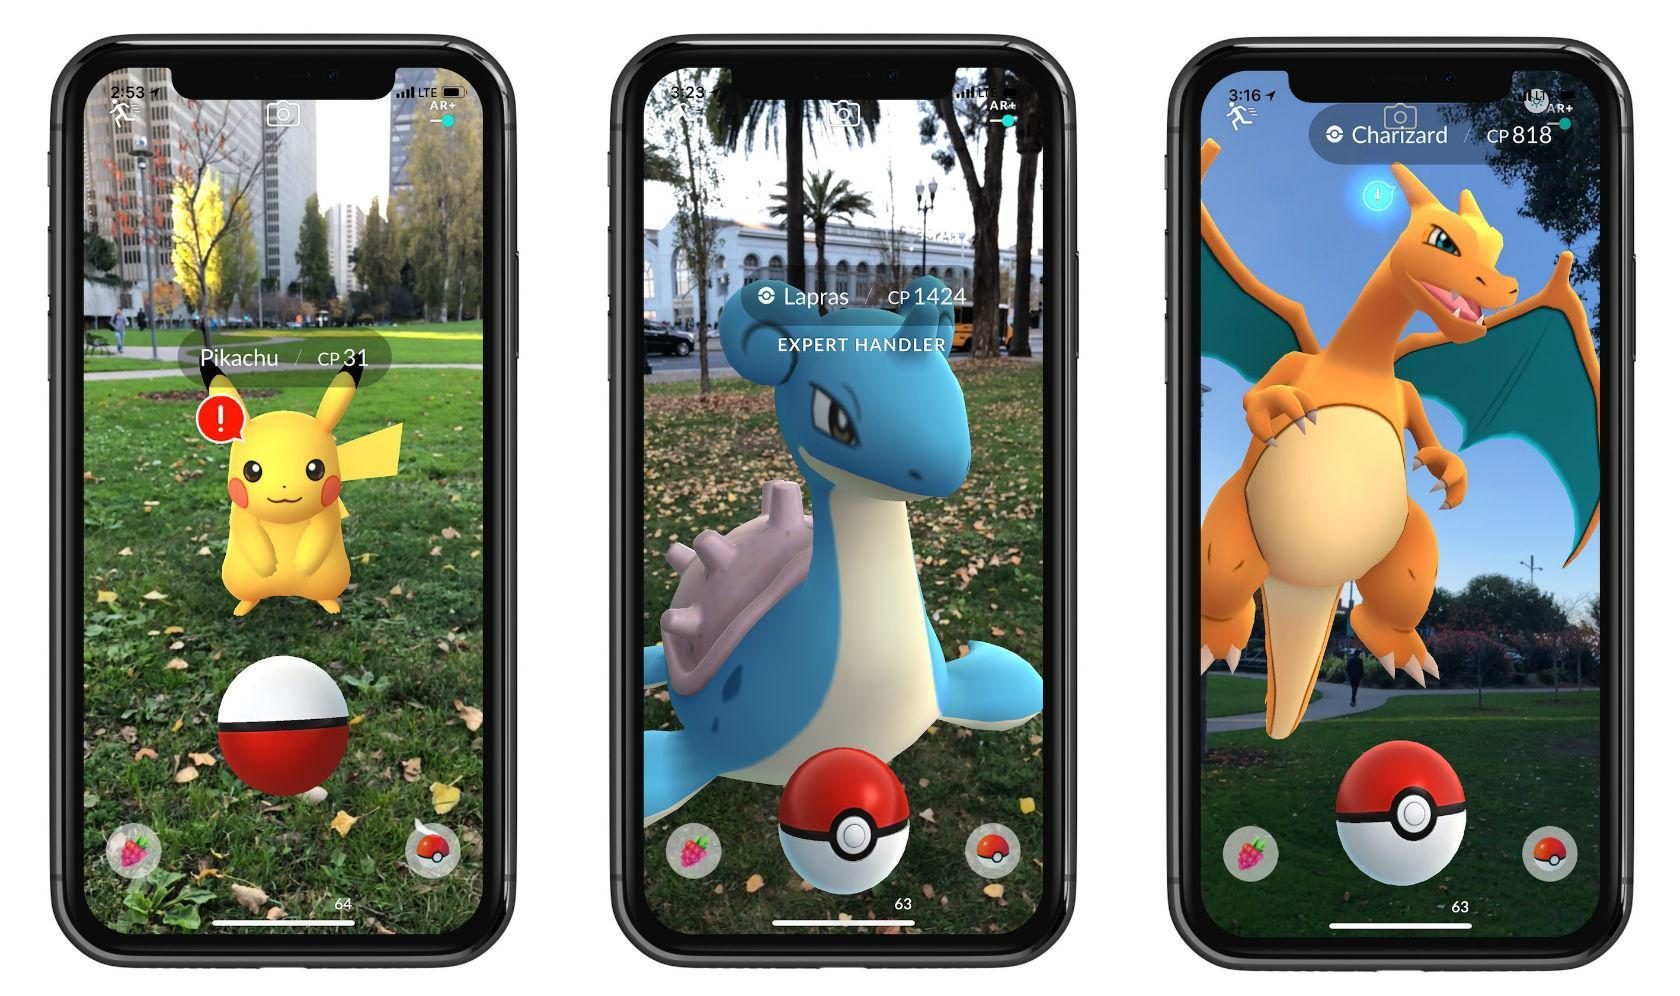
\includegraphics[width=0.7\textwidth]{Images/pokemon-go-arplus-iphone-x.jpg}
     \caption[Captura del juego Pokémon Go]{Captura del juego Pokémon Go\footnotemark.}
     \label{fig:pokemonGo}
 \end{figure}

Como hemos comentado antes, la gamificación de otros sectores como la educación es una realidad, y muchos de los juegos que vemos en estos ámbitos se valen de la realidad aumentada para proporcionar al usuario una experiencia de aprendizaje nueva y más satisfactoria.\\

El futuro en este campo es sin ninguna duda de los más prometedores, puesto que un alto porcentaje de los jugadores afirma que si se llegase a prescindir de las pantallas de dispositivos móviles para el despliegue de aplicaciones en realidad aumentada y se utilizasen visores más pequeños y cómodos de alta durabilidad y precio asequible, no dudarían en utilizar esta tecnología en su tiempo de ocio habitual~\cite{caracolRadio}.

\subsection{Comercio electrónico (\textit{e-commerce})}\label{ecommerce}
Los probadores virtuales están marcando tendencia en las nuevas generaciones de aplicaciones y estrategias de venta. Estas aplicaciones hacen uso de la realidad aumentada con tecnologías como el reconocimiento de rostros, reconocimiento de superficies o estimación de luces, y son punto de referencia en el mercado los siguientes ejemplos:
\begin{enumerate}[label={\arabic*.}]
\item \textbf{Ikea Place}\\
Esta aplicación permite al usuario ver el catálogo de Ikea y una vez seleccionado el elemento verlo en la habitación real con las dimensiones reales del objeto.
\begin{figure}[H]
     \centering
     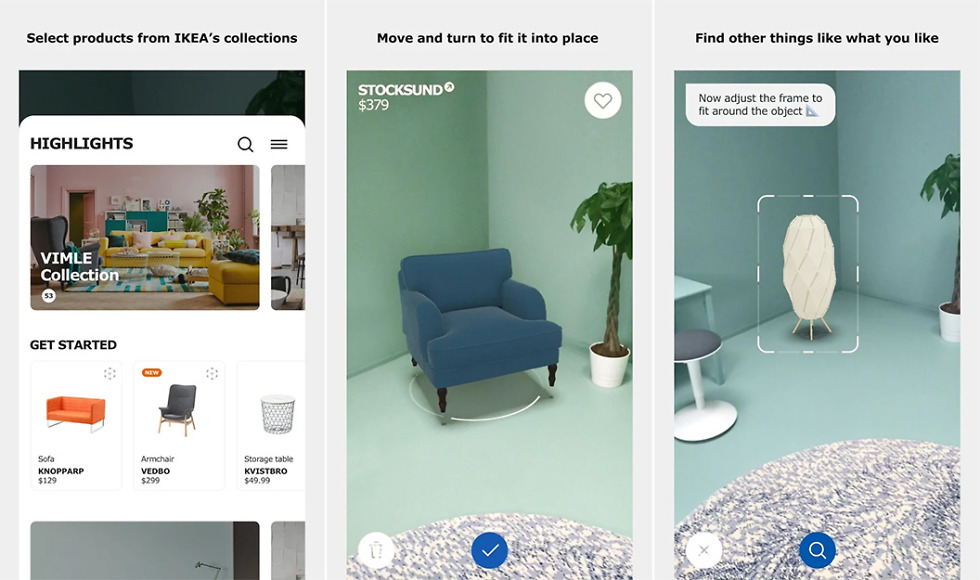
\includegraphics[width=0.5\textwidth]{Images/Ikea_App.jpeg}
     \caption[IKEA Place AR probador virtual]{IKEA Place AR probador virtual\footnotemark.}
     \label{fig:Ikea}
 \end{figure}
  \footnotetext{Imagen sacada de  \url{https://www.droid-life.com/wp-content/uploads/2018/03/ikea-place-android-app-980x580.jpg}}
 
 \item
 \textbf{YouCam Makeup}\\
Esta aplicación es un excelente y conseguido ejemplo de e-commerce en el mundo de la belleza donde se aplica esta tecnología. La calidad del \textit{tracking} del pelo es bastante precisa generando una experiencia agradable.
\begin{figure}[H]
    \centering
    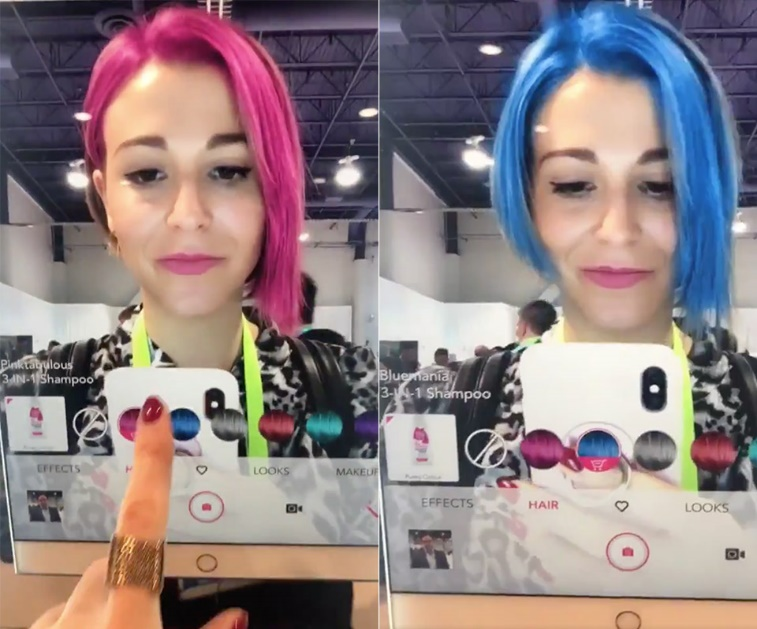
\includegraphics{Images/Loreal_App.jpeg}
    \caption[Imagen representativa de YouCam Makeup]{Imagen representativa de YouCam Makeup\footnotemark.}
    \label{fig:YouCam}
\end{figure}
 \footnotetext{Imagen sacada de \\ \url{https://www.techeblog.com/artificial-intelligence-software-hair-color-youcam-makeup-app/}}
\item \textbf{L’Oreal (Modiface)}\\
Esta Aplicación permite al usuario maquillarse con los productos de L’Oreal en realidad aumentada, así como escoger el color que mejor combine con sus prendas. Muestra los productos relacionados con esa tonalidad y ofrece la posibilidad de comprarlos dentro de la aplicación.
\end{enumerate}

\subsection*{Resumen}
Como se ha visto en este capítulo, la realidad aumentada ha ido creciendo y evolucionando desde 1950 con el prototipo de Sensorama hasta novedosas aplicaciones existentes en la actualidad.\\

En la actualidad la realidad aumentada está presente en multitud de sectores como la medicina, la educación, el arte, la publicidad, el turismo, la fabricación y los videojuegos. Ante el crecimiento y las posibilidades de esta tecnología se han en desarrollado diferentes librerías que pasaremos a analizar en el siguiente capítulo.\\

Por otro lado, para un correcto conocimiento y análisis de las funcionalidades de estas librerías, también estudiaremos en el siguiente capítulo las tecnologías implicadas en la realidad aumentada sin marcadores.\\


\noindent
